\chapter{जैवअकार्बनिक रसायन}\label{ch:b3:bioinorganic}

हमारा रक्त आयरन के कारण लाल है; हॉर्सशू केकड़े का रक्त अपनी शिराओं में रंगहीन होता है
और वायु में नीला हो जाता है, क्योंकि वह ऑक्सीजन को कॉपर पर वहन करता है। जीवन
मुट्ठी भर धातु आयनों का उपयोग उन कार्यों के लिए करता है जो कोई कार्बनिक समूह नहीं कर सकता: ऑक्सीजन को
उत्क्रमणीय रूप से बाँधना, एकल इलेक्ट्रॉनों को ले जाना, जल को विभाजित करना, नाइट्रोजन का अपचयन करना,
किसी जल अणु को इतना अम्लीय बनाना कि वह कार्बन डाइऑक्साइड पर आक्रमण कर सके। यह अध्याय
इन कार्यों को उपसहसंयोजन रसायन के औज़ारों से पढ़ता है: कठोर और \omterm{def:b3:bioinorganic:hsab}{मृदु
अम्ल}, लिगैंड क्षेत्र और चक्रण अवस्थाएँ, साम्य और दर नियम, और
औषधों के रूप में प्रयुक्त धातुओं के साथ समाप्त होता है।

\begin{recall}
द्वितीय वर्ष के खंड ने $\alpha$-ऐमीनो अम्लों, पार्श्व शृंखलाओं और पेप्टाइडों, न्यूक्लियोक्षारकों
और न्यूक्लियोटाइडों, उपसहसंयोजन संकुलों, लिगैंड क्षेत्रों, उच्च और निम्न चक्रण, तथा
कठोर और मृदु नाभिकरागियों और इलेक्ट्रॉनरागियों का विवेचन किया; प्रथम वर्ष के खंड ने संकुलन
स्थिरांकों और pL पैमाने का। \Cref{ch:b3:complex-spectra-magnetism} और
\cref{ch:b3:complex-mechanisms} ने स्पेक्ट्रम, मार्कस सिद्धांत और सिसप्लैटिन का
ऐक्वाकरण दिया, \cref{ch:b3:complex-kinetics} ने माइकेलिस--मेंटेन बलगतिकी, और
\cref{ch:b3:advanced-nmr} ने विश्रांति काल $T_1$।
\end{recall}

\begin{omfigure}
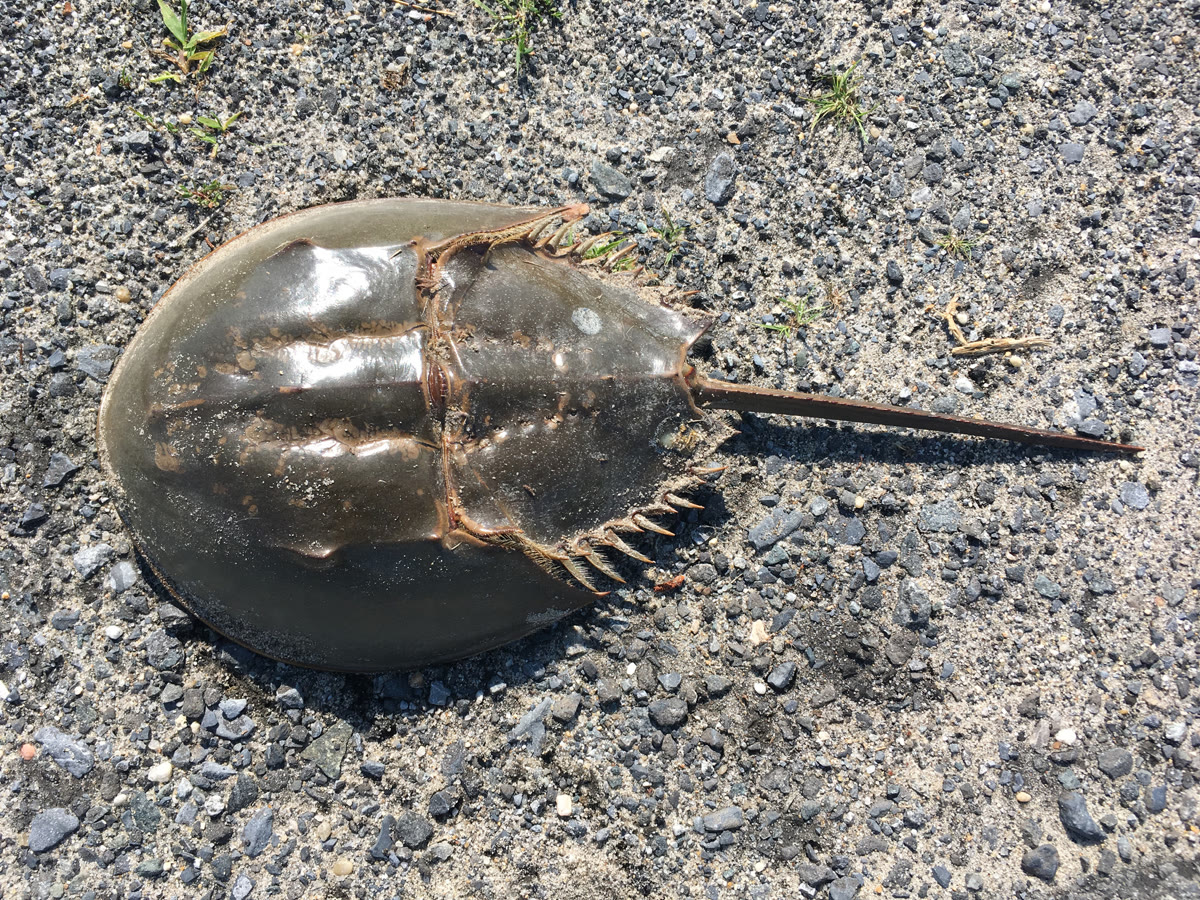
\includegraphics[width=0.5\linewidth]{images/book4/horseshoe-crab.jpg}

{\small एक अटलांटिक हॉर्सशू केकड़ा। इसका रक्त ऑक्सीजन को हीमोसायनिन, एक
कॉपर प्रोटीन, पर वहन करता है, और ऑक्सीजनित होने पर नीला होता है। छायाचित्र: कालदारी, CC0।}
\end{omfigure}

\section{जीवविज्ञान में धातुएँ}

\begin{definition}[धातुप्रोटीन]\label{def:b3:bioinorganic:metalloprotein}
\emph{धातुप्रोटीन}\index{धातुप्रोटीन} वह प्रोटीन है जिसमें
बँधे हुए धातु आयन होते हैं; \emph{धातुएंज़ाइम}\index{धातुएंज़ाइम} वह है जो
किसी अभिक्रिया को उत्प्रेरित करता है। \emph{सहकारक}\index{सहकारक} एक अप्रोटीन स्पीशीज़ है,
कोई धातु आयन या छोटा अणु, जो किसी प्रोटीन से बँधा हो और उसकी
सक्रियता के लिए आवश्यक हो।
\end{definition}

मात्रा में महत्त्वपूर्ण धातुएँ सोडियम, पोटैशियम, मैग्नीशियम और
कैल्सियम हैं, जो अधिकतर आवेश वहन करती हैं और संरचनाएँ थामती हैं; संक्रमण धातुएँ
आयरन, ज़िंक, कॉपर, मैंगनीज़, कोबाल्ट, मॉलिब्डेनम और निकेल अल्प मात्रा में होती हैं
पर रसायन का बड़ा भाग चलाती हैं। कोई प्रोटीन अपनी धातु का चयन उन दाता
परमाणुओं और उनकी ज्यामिति द्वारा करता है जो वह प्रस्तुत करता है।

\begin{definition}[कठोर और मृदु अम्ल]\label{def:b3:bioinorganic:hsab}
\emph{कठोर अम्ल}\index{कठोर अम्ल} एक छोटा, उच्च आवेशित, दुर्बल
ध्रुवणीय लुइस अम्ल है ($\ce{H+}$, $\ce{Mg^2+}$, $\ce{Ca^2+}$, $\ce{Fe^3+}$); \emph{मृदु
अम्ल}\index{मृदु अम्ल} कम आवेश वाला एक बड़ा, ध्रुवणीय अम्ल है ($\ce{Cu+}$, $\ce{Ag+}$,
$\ce{Hg^2+}$, $\ce{Cd^2+}$)। \emph{कठोर और मृदु अम्ल--क्षारक सिद्धांत}\index{कठोर और मृदु अम्ल--क्षारक सिद्धांत}
कहता है कि कठोर अम्ल वरीयता से कठोर क्षारकों
(ऑक्सीजन दाता, फ़्लुओराइड) से और मृदु अम्ल मृदु क्षारकों (सल्फ़र दाता, आयोडाइड) से बँधते हैं।
\end{definition}

प्रोटीनों में कार्बोक्सिलेट और फ़ीनॉलेट कठोर हैं, सिस्टीन का थायोलेट और
मेथियोनीन का थायोईथर मृदु, और हिस्टिडीन का इमिडैज़ोल बीच में। आयरन(III)
ऑक्सीजन दाताओं के बीच बैठता है, कॉपर(I) सल्फ़र दाताओं के बीच, ज़िंक, एक सीमांत
अम्ल, हिस्टिडीन और सिस्टीन के साथ; पारा और कैडमियम अंशतः इसलिए विषैले हैं
क्योंकि वे \omterm{def:b3:complex-kinetics:enzyme}{एंज़ाइमों} के सिस्टीनों को जकड़ लेते हैं।

\begin{definition}[अर्विंग--विलियम्स श्रेणी]\label{def:b3:bioinorganic:irving-williams}
\emph{अर्विंग--विलियम्स श्रेणी}\index{अर्विंग--विलियम्स श्रेणी} किसी दिए गए लिगैंड के साथ
प्रथम संक्रमण श्रेणी के द्विसंयोजी आयनों के उच्च-चक्रण संकुलों के स्थायित्व का
क्रम है:
$\ce{Mn^2+} < \ce{Fe^2+} < \ce{Co^2+} < \ce{Ni^2+} < \ce{Cu^2+} > \ce{Zn^2+}$।
\end{definition}

\begin{proposition}[अर्विंग--विलियम्स क्रम]\label{prop:b3:bioinorganic:irving-williams}
यह श्रेणी लगभग सभी लिगैंडों के लिए सत्य है (एक प्रायोगिक प्रेक्षण); यह
मैंगनीज़ से कॉपर तक आयनिक त्रिज्या की कमी, लिगैंड-क्षेत्र
स्थायीकरण ऊर्जा, जो $d^5$ के लिए शून्य और $d^8$ के लिए सबसे बड़ी है, और कॉपर(II) की यान--टेलर
विकृति का अनुसरण करती है, जो उसके चार आबंधों को छोटा कर देती है।
\end{proposition}

\begin{proof}[तर्क]
नाभिकीय आवेश बढ़ने के साथ पंक्ति में त्रिज्या घटती है, जिससे प्रत्येक लिगैंड का
स्थिरवैद्युत आकर्षण दृढ़ होता है। उच्च-चक्रण अष्टफलकीय आयनों का लिगैंड-क्षेत्र स्थायीकरण
(\cref{ch:b3:complex-spectra-magnetism}) $0$, $4$,
$8$, $12$ और $6\,\mathrm{Dq}$ है, $d^5$ से $d^9$ के लिए, और $0$, $d^{10}$ के लिए: यह निकेल तक प्रवृत्ति में जुड़ता है और
ज़िंक के लिए गिर जाता है; कॉपर(II) अपनी चतुष्कोणीय विकृति द्वारा, जो चार छोटे, दृढ़ आबंध देती है,
अपने स्थायीकरण के संकेत से अधिक लाभ प्राप्त करता है।
\end{proof}

कोशिकाओं को एक परिणाम का प्रबंधन करना पड़ता है: कॉपर और ज़िंक अधिकांश स्थलों के लिए
अन्य आयनों को पछाड़ देते, अतः विशिष्ट वाहक प्रोटीनों द्वारा उनकी मुक्त सांद्रताएँ
अत्यंत कम रखी जाती हैं।

\section{ऑक्सीजन परिवहन}

\begin{definition}[पॉर्फ़िरिन और हीम]\label{def:b3:bioinorganic:haem}
\emph{पॉर्फ़िरिन}\index{पॉर्फ़िरिन} चार पिरोल वलयों का एक बड़ा, समतल, ऐरोमैटिक बृहत्चक्र है,
जो मेथीन सेतुओं से जुड़े होते हैं, और जिसके चार नाइट्रोजन उसके केंद्र पर
एक धातु आयन को बाँधते हैं। \emph{हीम}\index{हीम} प्रोटोपॉर्फ़िरिन~IX का आयरन संकुल है,
जो हीमोग्लोबिन, मायोग्लोबिन और साइटोक्रोमों का \omterm{def:b3:bioinorganic:metalloprotein}{सहकारक} है।
\end{definition}

मायोग्लोबिन और हीमोग्लोबिन में \omterm{def:b3:bioinorganic:haem}{हीम} के आयरन का एक पाँचवाँ लिगैंड वलय के नीचे होता है,
समीपस्थ हिस्टिडीन का नाइट्रोजन, और छठा स्थल $\ce{O2}$ के लिए मुक्त रहता है।
विऑक्सी आयरन(II) उच्च चक्रण है: $d_{x^2-y^2}$ कक्षक में एक इलेक्ट्रॉन, जो चार
नाइट्रोजनों की ओर इंगित करता है, उसे वलय के छिद्र के लिए बहुत बड़ा बना देता है, और वह
तल से बाहर, हिस्टिडीन की ओर, बैठता है। $\ce{O2}$ से बँधने पर वह निम्न चक्रण, छोटा, हो जाता है, और
तल में आ जाता है, हिस्टिडीन और प्रोटीन कुंडलिनी को अपने साथ खींचते हुए।

\begin{omfigure}
% ledger: pdb:Hb.deoxy.FeN4, pdb:Hb.oxy.FeN4
\begin{tikzpicture}[font=\small, scale=0.9]
  \foreach \x/\lab/\dz/\oxy in {0/विऑक्सी (उच्च चक्रण)/-0.34/0, 6.4/ऑक्सी (निम्न चक्रण)/-0.04/1} {
    \begin{scope}[xshift=\x cm]
      \draw[omDef, line width=2.6pt] (-2.2,0) -- (2.2,0);
      \node[font=\scriptsize, anchor=west, omDef] at (2.3,0) {पॉर्फ़िरिन};
      \fill[omThm] (0,\dz*1.5) circle (0.22);
      \node[font=\scriptsize, anchor=north west] at (0.2,\dz*1.5-0.12) {Fe};
      \draw[black!70, line width=1pt] (0,\dz*1.5-0.22) -- (0,-1.55);
      \node[draw=black!70, regular polygon, regular polygon sides=5, minimum size=7mm, inner sep=0pt] at (0,-1.95) {};
      \node[font=\scriptsize, anchor=west] at (0.45,-1.95) {समीपस्थ His};
      \node[font=\small\bfseries] at (0,1.9) {\lab};
      \ifnum\oxy=1
        \draw[black!70, line width=1pt] (0,0.2) -- (0,0.85) -- (0.55,1.25);
        \fill[red!75] (0,0.85) circle (0.13) (0.55,1.25) circle (0.13);
        \node[font=\scriptsize, anchor=west] at (0.75,1.2) {$\ce{O2}$, मुड़ा हुआ};
      \fi
    \end{scope}
  }
  \draw[<->, black!60] (-1.0,0) -- (-1.0,-0.51) node[midway, left, font=\scriptsize] {\qty{0.34}{\angstrom}};
\end{tikzpicture}

{\small किनारे से देखा गया \omterm{def:b3:bioinorganic:haem}{हीम} आयरन, वलय से उसका विस्थापन पैमाने पर
दिखाया गया (1~\AA{} को 1.35~cm के रूप में; अन्य दूरियाँ व्यवस्थात्मक हैं)। विऑक्सीहीमोग्लोबिन में उच्च-चक्रण आयरन(II)
चार पिरोल नाइट्रोजनों के माध्य तल से \qty{0.34}{\angstrom} नीचे,
समीपस्थ हिस्टिडीन की ओर, स्थित है; ऑक्सीहीमोग्लोबिन में यह तल से \qty{0.05}{\angstrom} के भीतर है, $\ce{O2}$
सिरे से बँधा और मुड़ा हुआ (क्रिस्टल संरचनाओं से परिकलित दूरियाँ)।}
\end{omfigure}

बँधी हुई डाइऑक्सीजन का वर्णन आयरन(III) पर सुपरऑक्साइड, $\ce{Fe^{III}-O2^-}$, के रूप में बेहतर होता है, बजाय
आयरन(II) पर उदासीन $\ce{O2}$ के: संकुल प्रतिचुंबकीय है क्योंकि दोनों केंद्रों के अयुग्मित
इलेक्ट्रॉन युग्मित हो जाते हैं। प्रोटीन आयरन(III) और जल तक के अनुत्क्रमणीय
ऑक्सीकरण को रोकता है, जो जल में एक नग्न \omterm{def:b3:bioinorganic:haem}{हीम} तुरंत झेलता
है।

\begin{definition}[सहकारी बंधन]\label{def:b3:bioinorganic:cooperativity}
अनेक स्थलों वाले किसी प्रोटीन से बंधन \emph{सहकारी}\index{सहकारी बंधन} होता है
जब एक लिगैंड का बंधन शेष स्थलों की बंधुता बढ़ा
देता है। \emph{हिल गुणांक}\index{हिल गुणांक} $n$
हिल आलेख, $\log\frac{\theta}{1 - \theta}$ का $\log p$ के विरुद्ध, का अर्ध संतृप्ति पर ढलान है ($\theta$ अधिकृत स्थलों का
अंश है)।
\end{definition}

\begin{proposition}[एक स्थल]\label{prop:b3:bioinorganic:hyperbola}
एक स्थल वाले प्रोटीन के लिए, $\mathrm{P + O_2 \rightleftharpoons PO_2}$, अधिकृत अंश $\theta = p/(p_{50} + p)$ है, जहाँ $p_{50}$
दाब के रूप में व्यक्त वियोजन स्थिरांक है।
\end{proposition}

\begin{proof}
$K_d = [\mathrm P]p/[\mathrm{PO_2}] = p_{50}$, अतः $[\mathrm{PO_2}] = [\mathrm P]p/p_{50}$, और $\theta = [\mathrm{PO_2}]/([\mathrm P] + [\mathrm{PO_2}]) = (p/p_{50})/(1 + p/p_{50})$।
\end{proof}

\begin{theorem}[हिल समीकरण]\label{thm:b3:bioinorganic:hill}
$n$ स्थलों वाले ऐसे प्रोटीन के लिए जिसके स्थल या तो सब रिक्त हों या सब भरे,
$\mathrm{P + n\,O_2 \rightleftharpoons P(O_2)_n}$,
\[
  \theta = \frac{p^n}{p_{50}^n + p^n}, \qquad \log\frac{\theta}{1 - \theta} = n\log p - n\log p_{50}.
\]
\end{theorem}

\begin{proof}
$K_d = [\mathrm P]p^n/[\mathrm{P(O_2)_n}]$; $K_d = p_{50}^n$ लिखिए। अधिकृत स्थलों का अंश भरे रूप वाले
अणुओं का अंश है, $\theta = [\mathrm{P(O_2)_n}]/([\mathrm P] + [\mathrm{P(O_2)_n}]) = (p/p_{50})^n/(1 + (p/p_{50})^n)$। तब $\theta/(1 - \theta) = (p/p_{50})^n$, और
लघुगणक लेने पर ढलान $n$ की सीधी रेखा मिलती है।
\end{proof}

हीमोग्लोबिन, चार स्थलों के साथ, पूर्णतः \omterm{def:b3:bioinorganic:cooperativity}{सहकारी} नहीं है: उसका \omterm{def:b3:bioinorganic:cooperativity}{हिल गुणांक}
4 से काफ़ी नीचे, लगभग 3, है, और उसके हिल आलेख का ढलान दोनों छोरों पर 1 है, जहाँ
वह स्वतंत्र स्थलों वाले विऑक्सी या ऑक्सी प्रोटीन की तरह व्यवहार करता है।
सहकारिता चतुष्क संरचना के परिवर्तन से आती है: $\ce{O2}$ से बँधने वाले पहले \omterm{def:b3:bioinorganic:haem}{हीम} के तल में
आयरन की गति अन्य उप-इकाइयों तक पहुँचाई जाती है।

\begin{omfigure}
\begin{tikzpicture}
\begin{axis}[name=a, width=0.48\linewidth, height=5.6cm, xmin=0, xmax=14, ymin=0, ymax=1.02,
  axis lines=left, xlabel={$p(\ce{O2})$ / \unit{kPa}}, ylabel={संतृप्ति $\theta$},
  tick label style={font=\scriptsize}, label style={font=\small}]
\addplot[omMeth, thick] table[x=p, y=Mb] {figdata/out/bachelor-3-oxygen-binding.dat};
\addplot[omThm, thick] table[x=p, y=Hb] {figdata/out/bachelor-3-oxygen-binding.dat};
\addplot[omThm, thick, dashed] table[x=p, y=Hbacid] {figdata/out/bachelor-3-oxygen-binding.dat};
\draw[black!35] (axis cs:5,0) -- (axis cs:5,1.0) (axis cs:13,0) -- (axis cs:13,1.0);
\node[font=\scriptsize, anchor=south] at (axis cs:5,0.02) {ऊतक};
\node[font=\scriptsize, anchor=south east] at (axis cs:13,0.02) {फेफड़े};
\node[font=\scriptsize, omMeth] at (axis cs:1.9,0.96) {Mb};
\node[font=\scriptsize, omThm] at (axis cs:7.5,0.6) {Hb};
\end{axis}
\begin{axis}[at={(a.east)}, anchor=west, xshift=1.4cm, width=0.48\linewidth, height=5.6cm,
  xmin=-1.5, xmax=1.5, ymin=-3, ymax=3, axis lines=left,
  xlabel={$\log_{10}(p/\unit{kPa})$}, ylabel={$\log_{10}\bigl(\theta/(1-\theta)\bigr)$},
  tick label style={font=\scriptsize}, label style={font=\small}]
\draw[black!30] (axis cs:-1.5,0) -- (axis cs:1.5,0);
\addplot[omMeth, thick] table[x=lgp, y=Mb] {figdata/out/bachelor-3-oxygen-binding-b.dat};
\addplot[omThm, thick, restrict y to domain=-3:3] table[x=lgp, y=Hb] {figdata/out/bachelor-3-oxygen-binding-b.dat};
\node[font=\scriptsize, omMeth, anchor=west] at (axis cs:-1.1,1.4) {ढलान 1};
\node[font=\scriptsize, omThm, anchor=west] at (axis cs:0.75,-1.5) {ढलान 2.7};
\end{axis}
\end{tikzpicture}

{\small बाएँ: मायोग्लोबिन (हरा) और हीमोग्लोबिन (लाल;
धराशायी: निम्नतर pH पर) की ऑक्सीजन संतृप्ति, ऑक्सीजन के दाब के विरुद्ध, मॉडल मानों
$p_{50} = \qty{0.37}{kPa}$ (Mb) और \qty{3.5}{kPa} (Hb), $n = 2.7$ के साथ। फेफड़ों और ऊतकों के बीच हीमोग्लोबिन
अपनी ऑक्सीजन का एक-चौथाई छोड़ देता है, मायोग्लोबिन लगभग कुछ नहीं। दाएँ: संगत
हिल आलेख, इस मॉडल में सीधी रेखाएँ (वास्तविक हीमोग्लोबिन का आलेख
दोनों छोरों पर ढलान 1 की ओर मुड़ता है)।}
\end{omfigure}

\begin{method}[हिल आलेख पढ़ना]\label{met:b3:bioinorganic:hill-plot}
\begin{enumerate}
  \item प्रत्येक मापी गई संतृप्ति से $\log(\theta/(1 - \theta))$ परिकलित कीजिए; इसे $\log p$ के विरुद्ध आलेखित कीजिए।
  \item जिस दाब पर आलेख शून्य को काटता है वह $p_{50}$ है।
  \item उस बिंदु पर ढलान \omterm{def:b3:bioinorganic:cooperativity}{हिल गुणांक} है: $n = 1$ का अर्थ स्वतंत्र
        स्थल, $n > 1$ \omterm{def:b3:bioinorganic:cooperativity}{सहकारी बंधन}।
  \item केवल दो बिंदुओं के साथ, $n = \Delta\log(\theta/(1 - \theta))/\Delta\log p$।
\end{enumerate}
\end{method}

हीमोग्लोबिन \omterm{def:b3:bioinorganic:haem}{हीम} से दूर स्थलों पर प्रोटॉनों और कार्बन डाइऑक्साइड को भी बाँधता है,
जो उसके वक्र को वहाँ दाईं ओर खिसका देते हैं जहाँ वे प्रचुर हैं, अर्थात् कार्यरत ऊतकों में:
बोर प्रभाव ठीक वहीं अधिक ऑक्सीजन मुक्त करता है जहाँ उसकी आवश्यकता है।

\begin{proposition}[कार्बन मोनोऑक्साइड स्पर्धा]\label{prop:b3:bioinorganic:haldane}
यदि कार्बन मोनोऑक्साइड और डाइऑक्सीजन एक ही स्थलों के लिए स्पर्धा करें,
$\mathrm{HbO_2 + CO \rightleftharpoons HbCO + O_2}$ के साथ, जिसका साम्य स्थिरांक $M$ है, तो
$[\mathrm{HbCO}]/[\mathrm{HbO_2}] = M\,p(\ce{CO})/p(\ce{O2})$।
\end{proposition}

\begin{proof}
साम्य पर $M = [\mathrm{HbCO}]\,p(\ce{O2})/([\mathrm{HbO_2}]\,p(\ce{CO}))$; पुनर्व्यवस्थित करने पर परिणाम मिलता है।
\end{proof}

मानव हीमोग्लोबिन के लिए $M$ सैकड़ों में है, अतः कार्बन मोनोऑक्साइड के कुछ सौ भाग प्रति
दस लाख स्थलों के एक बड़े अंश को घेर लेते हैं; इससे भी बुरा, मुक्त बचे
स्थल अपनी ऑक्सीजन को और दृढ़ता से थामे रखते हैं, क्योंकि सहकारिता
उन पर कार्य करती है। मुक्त \omterm{def:b3:bioinorganic:haem}{हीम} कार्बन मोनोऑक्साइड को और भी कहीं अधिक प्रबलता से बाँधता है:
प्रोटीन में आयरन के ऊपर एक दूरस्थ हिस्टिडीन उस रैखिक Fe--C--O
ज्यामिति में बाधा डालता है जिसे कार्बन मोनोऑक्साइड पसंद करता है, जबकि वह मुड़े हुए $\ce{O2}$ से हाइड्रोजन आबंध बनाता है।
अन्य जंतु अन्य धातुओं का उपयोग करते हैं: मोलस्कों और संधिपादों के हीमोसायनिन
$\ce{O2}$ को दो कॉपर आयनों के बीच पेरॉक्साइड के रूप में बाँधते हैं, कुछ समुद्री
कृमियों के हीमएरिथ्रिन आयरन आयनों के एक युग्म पर।

\begin{inthelab}[एक ऑक्सीजन-बंधन वक्र]
बफ़र में हीमोग्लोबिन का एक विलयन, एक पार्श्व फ़्लास्क से युक्त, गैस-रोधी क्यूवेट में
रखा जाता है। पहले नाइट्रोजन प्रवाहित करके उसे ऑक्सीजन से मुक्त किया जाता है, फिर
वायु के ज्ञात आयतन अंतःक्षिप्त किए जाते हैं और हल्के से झुकाकर विलयन को साम्यित किया जाता है।
प्रत्येक योग के बाद दृश्य स्पेक्ट्रम अभिलिखित किया जाता है: विऑक्सी रूप के बैंड
(लगभग \qty{555}{nm} पर एक बैंड) ऑक्सी रूप के दो बैंडों में बदल जाते हैं,
और संतृप्ति एक तरंगदैर्ध्य पर अवशोषकता से, उसकी
विऑक्सी और ऑक्सी सीमाओं के बीच, पढ़ी जाती है।
\end{inthelab}

\section{धातुएंज़ाइम}

कार्बोनिक ऐनहाइड्रेज़ $\ce{CO2 + H2O <=> HCO3- + H+}$ को तेज़ करता है, जो अकेले जल में
कुछ सेकंड लेती है, जो फेफड़े की केशिका से लाल कोशिका के छोटे से गमन में महत्त्वपूर्ण होने के लिए
पर्याप्त है। इसका ज़िंक आयन तीन हिस्टिडीनों और एक जल अणु द्वारा थामा जाता है।
उच्च आवेश का एक छोटा धनायन होने के नाते, यह उस जल का $\mathrm pK_a$ लगभग 14 से
लगभग 7 तक घटा देता है: शरीरक्रियात्मक pH पर \omterm{def:b3:complex-kinetics:enzyme}{एंज़ाइम} के एक अच्छे भाग पर ज़िंक-बद्ध
हाइड्रॉक्साइड होता है, एक प्रबल नाभिकरागी, जो $\ce{CO2}$ बाँधने वाली एक जेब के ठीक बगल में रहता है।

\begin{omfigure}
\begin{tikzpicture}[font=\small, >=Stealth]
  \node (a) at (90:2.0) {$\mathrm{(His)_3Zn{-}OH_2}$};
  \node (b) at (0:2.9) {$\mathrm{(His)_3Zn{-}OH^-}$};
  \node (c) at (-90:2.0) {$\mathrm{(His)_3Zn{-}OCO_2H^-}$};
  \draw[->, thick] (a) to[bend left=25] node[midway, above right, font=\scriptsize] {$-\,\ce{H+}$ (एक हिस्टिडीन शटल को)} (b);
  \draw[->, thick] (b) to[bend left=25] node[midway, below right, font=\scriptsize, align=left] {$+\,\ce{CO2}$:\\ नाभिकरागी आक्रमण} (c);
  \draw[->, thick] (c) to[bend left=35] node[midway, left, font=\scriptsize, align=right] {$+\,\ce{H2O}$\\ $-\,\ce{HCO3-}$} (a);
\end{tikzpicture}

{\small कार्बोनिक ऐनहाइड्रेज़ का उत्प्रेरकी चक्र। ज़िंक-बद्ध जल एक
प्रोटॉन खोता है; ज़िंक-बद्ध हाइड्रॉक्साइड कार्बन डाइऑक्साइड पर आक्रमण करता है; जल
हाइड्रोजनकार्बोनेट को विस्थापित करता है। विलायक को प्रोटॉन स्थानांतरण सबसे धीमा चरण है।}
\end{omfigure}

\begin{proposition}[एक तीव्र एंज़ाइम]\label{prop:b3:bioinorganic:carbonic-anhydrase}
कार्बोनिक ऐनहाइड्रेज़ का \omterm{def:b3:complex-kinetics:michaelis}{विशिष्टता स्थिरांक} $k_{\mathrm{cat}}/K_M$, \omterm{def:b3:complex-kinetics:enzyme}{एंज़ाइम} के साथ $\ce{CO2}$ की भेंट के
दर स्थिरांक के निकट पहुँचता है: लगभग हर भेंट
अभिक्रिया तक ले जाती है।
\end{proposition}

\begin{proof}[तर्क]
$k_{\mathrm{cat}}/K_M$ निम्न क्रियाधार सांद्रता पर \omterm{def:b3:complex-kinetics:enzyme}{एंज़ाइम} और क्रियाधार का द्वितीय-कोटि दर स्थिरांक है
(\cref{ch:b3:complex-kinetics}); यह उनकी भेंट के
\omterm{def:b3:rate-theories:diffusion}{विसरण-नियंत्रित} दर स्थिरांक से अधिक नहीं हो सकता
(\cref{ch:b3:rate-theories})। कार्बोनिक ऐनहाइड्रेज़ के मापे गए मान
किसी भी \omterm{def:b3:complex-kinetics:enzyme}{एंज़ाइम} के लिए ज्ञात उच्चतम मानों में हैं और उस सीमा के निकट हैं: तब \omterm{def:b3:complex-kinetics:enzyme}{सक्रिय स्थल} के भीतर का
रसायन दर को सीमित करने वाला नहीं रहता।
\end{proof}

यकृत और अनेक अन्य कोशिकाओं में साइटोक्रोम P450 \omterm{def:b3:complex-kinetics:enzyme}{एंज़ाइम} औषधों और हॉर्मोनों के C--H
आबंधों का हाइड्रॉक्सिलन करते हैं। उनका \omterm{def:b3:bioinorganic:haem}{हीम} आयरन एक सिस्टीन थायोलेट द्वारा थामा जाता है;
$\ce{O2}$ और दो इलेक्ट्रॉनों के साथ यह \omterm{def:b3:bioinorganic:haem}{पॉर्फ़िरिन} पर एक मूलक सहित आयरन(IV)-ऑक्सो संकुल बनाता है,
जिसे यौगिक I कहते हैं, जो क्रियाधार से एक हाइड्रोजन परमाणु का
अपहरण करता है और हाइड्रॉक्सिल समूह को कार्बन मूलक पर लौटा देता है। नाइट्रोजिनेज़
कक्ष ताप पर $\ce{N2}$ को अमोनिया में अपचयित करता है, सात आयरन परमाणुओं, एक मॉलिब्डेनम
और नौ सल्फ़ाइडों के एक गुच्छ पर जो एक केंद्रीय कार्बन परमाणु के चारों ओर है, अर्थात् FeMo
\omterm{def:b3:bioinorganic:metalloprotein}{सहकारक}, ATP के अनेक अणुओं की कीमत पर। विटामिन $\mathrm{B_{12}}$ में एक
कोबाल्ट--कार्बन आबंध होता है, जीवविज्ञान के बहुत कम धातु--कार्बन आबंधों में से एक, जिसका
समांश विखंडन मूलक पुनर्विन्यास आरंभ करता है।

\section{इलेक्ट्रॉन स्थानांतरण और ऊर्जा}

जो प्रोटीन केवल इलेक्ट्रॉनों को ले जाते हैं उनके धातु केंद्रों की
\omterm{def:b3:complex-mechanisms:reorganisation}{पुनर्गठन ऊर्जा} छोटी होती है (\cref{ch:b3:complex-mechanisms}): दोनों ऑक्सीकरण
अवस्थाओं की ज्यामिति लगभग समान होती है, अतः मार्कस अवरोध निम्न होता है।

\begin{definition}[आयरन--सल्फ़र गुच्छ]\label{def:b3:bioinorganic:fes}
\emph{आयरन--सल्फ़र गुच्छ}\index{आयरन--सल्फ़र गुच्छ} आयरन
आयनों का एक समूह है जो सल्फ़ाइड आयनों द्वारा सेतुबद्ध और सिस्टीन थायोलेटों द्वारा प्रोटीन से बँधा होता है:
$\ce{[2Fe-2S]}$, $\ce{[3Fe-4S]}$ और घनाकार-सदृश $\ce{[4Fe-4S]}$।
\end{definition}

\begin{definition}[नीले कॉपर प्रोटीन]\label{def:b3:bioinorganic:blue-copper}
\emph{नीला कॉपर प्रोटीन}\index{नीला कॉपर प्रोटीन} एक विकृत चतुष्फलकीय स्थल में
दो हिस्टिडीनों, एक सिस्टीन और एक दुर्बल रूप से बँधे मेथियोनीन द्वारा बँधा एक कॉपर
आयन धारण करता है; इसका गहरा नीला रंग
सिस्टीन-से-कॉपर(II) आवेश-स्थानांतरण बैंड से आता है।
\end{definition}

\begin{definition}[एंटैटिक अवस्था]\label{def:b3:bioinorganic:entatic}
\emph{एंटैटिक अवस्था}\index{एंटैटिक अवस्था} वह धातु स्थल है जिसे
प्रोटीन एक तनावग्रस्त ज्यामिति में, उसकी दोनों ऑक्सीकरण अवस्थाओं द्वारा पसंद की जाने वाली
ज्यामितियों के बीच, थामे रखता है, जिससे उसकी अभिक्रियाओं की \omterm{def:b3:complex-mechanisms:reorganisation}{पुनर्गठन ऊर्जा} घटती है।
\end{definition}

अकेला कॉपर(II) वर्ग तल पसंद करता है, कॉपर(I) चतुष्फलक: नीले
कॉपर स्थल में दोनों में से कोई संतुष्ट नहीं होता, और इलेक्ट्रॉन स्थानांतरण तीव्र होता है।

\begin{definition}[ऑक्सीजन-मुक्तकारी संकुल]\label{def:b3:bioinorganic:oec}
प्रकाशतंत्र~II का \emph{ऑक्सीजन-मुक्तकारी संकुल}\index{ऑक्सीजन-मुक्तकारी संकुल}
वह $\mathrm{Mn_4CaO_5}$ गुच्छ है जो प्रकाश-संश्लेषण में जल को डाइऑक्सीजन में
ऑक्सीकृत करता है।
\end{definition}

\begin{proposition}[प्रति ऑक्सीजन चार फ़ोटॉन]\label{prop:b3:bioinorganic:kok}
दो जल अणुओं को एक $\ce{O2}$ में ऑक्सीकृत करने के लिए प्रकाशतंत्र~II द्वारा
अवशोषित चार फ़ोटॉन चाहिए, जबकि गुच्छ पाँच अवस्थाओं $\mathrm S_0$ से $\mathrm S_4$ से होकर गुज़रता है।
\end{proposition}

\begin{proof}
$\ce{2H2O -> O2 + 4H+ + 4e-}$: चार इलेक्ट्रॉन हटाने होते हैं। अभिक्रिया केंद्र द्वारा अवशोषित प्रत्येक फ़ोटॉन
उससे एक इलेक्ट्रॉन दूर ले जाता है, और गुच्छ ऑक्सीकृत केंद्र को
एक बार में एक इलेक्ट्रॉन से भरता है: चार फ़ोटॉन, चार चरण, जो
अवस्थाओं $\mathrm S_1$ से $\mathrm S_4$ में ऑक्सीकारी तुल्यांक संचित करते हैं; $\mathrm S_4$, $\ce{O2}$ मुक्त करके $\mathrm S_0$ पर लौटती है।
\end{proof}

\begin{omfigure}
\begin{tikzpicture}[font=\small, >=Stealth]
  \foreach \i/\ang in {0/90, 1/18, 2/-54, 3/-126, 4/162} {
    \node[draw, circle, minimum size=9mm, fill=omDef!10] (s\i) at (\ang:2.0) {$\mathrm S_{\i}$};
  }
  \foreach \i/\j in {0/1, 1/2, 2/3, 3/4} {
    \draw[->, thick] (s\i) to[bend left=18] node[midway, sloped, above, font=\scriptsize] {$h\nu$, $-\mathrm e^-$} (s\j);
  }
  \draw[->, thick, omThm] (s4) to[bend left=18] node[midway, sloped, above, font=\scriptsize] {$-\ce{O2}$, $+\,\ce{2H2O}$} (s0);
\end{tikzpicture}

{\small \omterm{def:b3:bioinorganic:oec}{ऑक्सीजन-मुक्तकारी संकुल} का कॉक चक्र। प्रकाशतंत्र~II द्वारा अवशोषित प्रत्येक फ़ोटॉन
मैंगनीज़ गुच्छ से एक इलेक्ट्रॉन हटाता है (प्रोटॉन
मार्ग में निकल जाते हैं); चौथा ऑक्सीकरण $\mathrm S_4$ देता है, जो डाइऑक्सीजन मुक्त करता है और
फिर से दो जल अणु बाँधता है।}
\end{omfigure}

ऊर्जा शृंखला के दूसरे छोर पर, सूत्रकणिकाओं का साइटोक्रोम $c$ ऑक्सीडेज़
एक-दूसरे के सामने स्थित एक \omterm{def:b3:bioinorganic:haem}{हीम} आयरन और एक कॉपर आयन पर चार इलेक्ट्रॉनों और चार प्रोटॉनों से
$\ce{O2}$ को जल में अपचयित करता है, आंशिक रूप से अपचयित, हानिकारक सुपरऑक्साइड या पेरॉक्साइड
मुक्त किए बिना।

\section{चिकित्सा में धातुएँ}

\begin{definition}[धातु-औषधें]\label{def:b3:bioinorganic:metallodrug}
\emph{धातु-औषध}\index{धातु-औषध} वह औषध है जिसकी सक्रियता किसी
धातु आयन या धातु संकुल पर निर्भर करती है।
\end{definition}

सिसप्लैटिन, \textit{cis}-$\ce{[PtCl2(NH3)2]}$, रक्त में स्थायी है, जहाँ क्लोराइड सांद्रता
ऊँची है; कोशिकाओं के भीतर, जहाँ यह कहीं कम है, यह एक क्लोराइड का जल से विनिमय करता है
(\cref{ch:b3:complex-mechanisms})। ऐक्वा संकुल ग्वानीन के N7 परमाणु से बँधता है,
फिर उसी रज्जुक पर उसके बगल वाले दूसरे ग्वानीन से: 1,2-GG
तिर्यक-बंध DNA को मोड़ देता है, जिसकी मरम्मत कोशिका नहीं कर पाती, और वह मर जाती है।
\textit{trans} समावयवी दो पड़ोसी क्षारकों को सेतुबद्ध नहीं कर सकता और निष्क्रिय है।
कार्बोप्लैटिन, धीरे निकलने वाले एक कीलेटी डाइकार्बोक्सिलेट के साथ, कम
दुष्प्रभाव देता है; ऑक्सैलिप्लैटिन, एक डाइऐमीनोसाइक्लोहेक्सेन लिगैंड के साथ, सिसप्लैटिन-प्रतिरोधी
अर्बुदों पर कार्य करता है।

\begin{omfigure}
\begin{tikzpicture}[font=\small]
  \draw[black!60, line width=1.4pt] (-3.2,0) -- (3.2,0);
  \node[font=\scriptsize, anchor=west] at (3.3,0) {DNA रज्जुक};
  \foreach \x/\b in {-2.4/C, -1.0/G, 1.0/G, 2.4/T} {
    \draw[black!60, line width=1pt] (\x,0) -- (\x,0.6);
    \node[draw=black!70, fill=white, rounded corners=1pt, minimum width=6mm] (n\b\x) at (\x,0.9) {\b};
  }
  \node (pt) at (0,2.4) {$\ce{Pt}$};
  \draw[omThm, thick] (pt) -- (-0.95,1.2) node[midway, left, font=\scriptsize] {N7};
  \draw[omThm, thick] (pt) -- (0.95,1.2) node[midway, right, font=\scriptsize] {N7};
  \draw (pt) -- (-0.5,3.1) node[above left, font=\scriptsize, inner sep=1pt] {$\ce{H3N}$};
  \draw (pt) -- (0.5,3.1) node[above right, font=\scriptsize, inner sep=1pt] {$\ce{NH3}$};
\end{tikzpicture}

{\small सिसप्लैटिन द्वारा बना 1,2-अंतःरज्जुक तिर्यक-बंध, व्यवस्थात्मक: अपने दो
क्लोराइड खोने के बाद प्लैटिनम एक रज्जुक के दो संलग्न ग्वानीनों के N7 परमाणुओं से
बँधता है, अपने दोनों \textit{cis} ऐम्मीन लिगैंडों को बनाए रखते हुए। वास्तविक योगज
द्विकुंडलिनी को मोड़ देता है।}
\end{omfigure}

\begin{definition}[विपर्यास कारक]\label{def:b3:bioinorganic:contrast}
चुंबकीय अनुनाद प्रतिबिंबन के लिए \emph{विपर्यास कारक}\index{विपर्यास कारक}
एक अनुचुंबकीय यौगिक है जो निकटवर्ती जल प्रोटॉनों के विश्रांति कालों को छोटा कर देता है।
इसकी \emph{विश्रांतिता}\index{विश्रांतिता} $r_1$ कारक की प्रति इकाई सांद्रता
विश्रांति दर $1/T_1$ में वृद्धि है।
\end{definition}

\begin{proposition}[विश्रांति दर]\label{prop:b3:bioinorganic:relaxivity}
\omterm{def:b3:bioinorganic:contrast}{विश्रांतिता} $r_1$ वाले कारक के साथ, सांद्रता $c$ पर, जल
प्रोटॉनों की विश्रांति दर $1/T_1 = 1/T_{1,0} + r_1c$ है, जहाँ $T_{1,0}$ कारक के बिना मान है।
\end{proposition}

\begin{proof}
अनुचुंबकीय योगदान उन कारक अणुओं की संख्या के समानुपाती है जिनसे
जल अणु प्रति इकाई समय मिलते हैं, अतः $c$ के समानुपाती; स्वतंत्र क्रियाविधियों की
विश्रांति दरें जुड़ती हैं। $r_1$ की परिभाषा से जुड़ी हुई दर $r_1c$ है।
\end{proof}

गैडोलिनियम(III), सात अयुग्मित इलेक्ट्रॉनों और धीरे विश्रांत होने वाले इलेक्ट्रॉन चक्रण वाला
$4f^7$, पसंदीदा धातु है। मुक्त $\ce{Gd^3+}$ विषैला है: इसे एक अष्टदंतुर
पॉलीऐमीनोकार्बोक्सिलेट के अत्यंत स्थायी संकुल के रूप में दिया जाता है जो एक जल अणु के लिए एक
स्थल छोड़ता है, जो स्थूल जल से तेज़ी से विनिमय करता है और विश्रांति को
पूरे जल तक पहुँचाता है।

\begin{definition}[कीलेटन चिकित्सा]\label{def:b3:bioinorganic:chelation-therapy}
\emph{कीलेटन चिकित्सा}\index{कीलेटन चिकित्सा} औषध के रूप में दिए गए एक कीलेटी लिगैंड द्वारा
शरीर से किसी विषैली धातु को हटाना है, जो एक स्थायी,
विलेय संकुल बनाता है जो उत्सर्जित हो जाता है।
\end{definition}

\begin{method}[कीलेटी औषध का चयन]\label{met:b3:bioinorganic:choose-chelator}
\begin{enumerate}
  \item विषैली धातु के साथ, और बड़ी मात्रा में उपस्थित आवश्यक धातुओं ($\ce{Ca^2+}$, $\ce{Mg^2+}$,
        $\ce{Zn^2+}$) के साथ कीलेटक के स्थायित्व स्थिरांकों की तुलना कीजिए।
  \item शरीर की सांद्रताओं और pH पर कीलेटक द्वारा छोड़ा गया मुक्त धातु स्तर $\mathrm{pM} = -\log[\mathrm M]$
        परिकलित कीजिए: विषैली धातु के लिए pM जितना ऊँचा और
        आवश्यक धातुओं के लिए जितना कम, उतना बेहतर।
  \item कीलेटक को स्पर्धी आवश्यक आयन से पहले ही भरकर दीजिए (सीसे के लिए EDTA का
        कैल्सियम संकुल), ताकि वह रक्त से कैल्सियम छीनने के बजाय
        विनिमय करे।
  \item कठोर--मृदु मेल (पारे और सीसे के लिए सल्फ़र दाता, आयरन(III) के लिए कठोर
        ऑक्सीजन दाता) और संकुल के उत्सर्जित होने की जाँच कीजिए।
\end{enumerate}
\end{method}

\begin{safety}{\ghs[0.62cm]{GHS05}\ghs[0.62cm]{GHS06}\ghs[0.62cm]{GHS08}}
% ledger: ghs4:cisplatin
सिसप्लैटिन: निगलने पर घातक, कैंसर और आनुवंशिक दोष उत्पन्न कर सकता है, प्रजनन क्षमता को
क्षति पहुँचा सकता है, आँखों को गंभीर क्षति और एलर्जी अभिक्रियाएँ उत्पन्न करता है; इसे
केवल तैयार औषध विलयन के रूप में, दस्ताने पहनकर, संवातित कैबिनेट में सँभाला जाता है।
\end{safety}

\begin{history}[एक प्रोटीन संरचना और एक संयोगवश मिली औषध]
मैक्स पेरुत्ज़ ने बीस से अधिक वर्षों तक हीमोग्लोबिन की X-किरण संरचना पर कार्य किया,
जो 1959 में निम्न विभेदन पर हल हुई; जॉन केंड्रू के साथ, जिन्होंने
मायोग्लोबिन हल किया, उन्हें रसायन का 1962 का नोबेल पुरस्कार मिला। 1965 में बार्नेट
रोज़ेनबर्ग ने, जीवाणुओं के एक संवर्धन में प्लैटिनम इलेक्ट्रोडों के बीच धारा प्रवाहित करते हुए,
उन्हें विभाजित हुए बिना लंबे तंतुओं में बढ़ते देखा; कारण
धारा नहीं, बल्कि इलेक्ट्रोडों से बना एक प्लैटिनम ऐम्मीन संकुल था। यही
सिसप्लैटिन बना, जो आज भी सबसे अधिक प्रयुक्त कैंसररोधी औषधों में से एक है।
\end{history}

\section{अभ्यास}

\begin{exercise}[$\star$]\label{exo:b3:bioinorganic:1}
एक प्रोटीन \qty{2.1}{kPa} ऑक्सीजन पर 20\,\% और \qty{5.9}{kPa} पर 80\,\% संतृप्त है। उसका
\omterm{def:b3:bioinorganic:cooperativity}{हिल गुणांक} परिकलित कीजिए।
\end{exercise}

\begin{exercise}[$\star$]\label{exo:b3:bioinorganic:2}
$\ce{Zn^2+}$, $\ce{Mn^2+}$, $\ce{Cu^2+}$, $\ce{Fe^2+}$, $\ce{Ni^2+}$ और $\ce{Co^2+}$ को किसी दिए गए लिगैंड के साथ उनके संकुलों के स्थायित्व के क्रम में
रखिए, और ज़िंक के स्थान की व्याख्या कीजिए।
\end{exercise}

\begin{exercise}[$\star$]\label{exo:b3:bioinorganic:3}
$\ce{Ca^2+}$, $\ce{Fe^3+}$, $\ce{Cu+}$, $\ce{Zn^2+}$ और $\ce{Hg^2+}$ के पसंदीदा प्रोटीन दाताओं (कार्बोक्सिलेट, सिस्टीन थायोलेट,
हिस्टिडीन इमिडैज़ोल) का पूर्वानुमान कीजिए।
\end{exercise}

\begin{exercise}[$\star$]\label{exo:b3:bioinorganic:4}
मुक्त हुए $\ce{O2}$ के प्रति अणु कितने इलेक्ट्रॉन हटाए जाते हैं, और प्रकाशतंत्र~II द्वारा कितने फ़ोटॉन
अवशोषित होते हैं? प्रति मोल?
\end{exercise}

\begin{exercise}[$\star\star$]\label{exo:b3:bioinorganic:5}
अध्याय के मॉडल वक्रों (मायोग्लोबिन के लिए $p_{50} = \qty{0.37}{kPa}$; हीमोग्लोबिन के लिए \qty{3.5}{kPa} और $n = 2.7$) के साथ,
\qty{13}{kPa} (फेफड़े) और \qty{5}{kPa} (ऊतक) के बीच प्रत्येक प्रोटीन अपनी ऑक्सीजन का कितना अंश छोड़ता है,
परिकलित कीजिए।
\end{exercise}

\begin{exercise}[$\star\star$]\label{exo:b3:bioinorganic:6}
\qty{50}{ppm} कार्बन मोनोऑक्साइड वाली वायु में इतनी देर तक साँस ली जाती है कि
साम्य स्थापित हो जाए। $M = 230$ (अभ्यास के आँकड़े) और वायु के $p(\ce{O2})/p(\ce{CO})$ के साथ
(20.95\,\% ऑक्सीजन), हीमोग्लोबिन का कितना अंश CO वहन करता है?
\end{exercise}

\begin{exercise}[$\star\star$]\label{exo:b3:bioinorganic:7}
गुच्छों $\ce{[Fe2S2(SR)4]^2-}$,
$\ce{[Fe2S2(SR)4]^3-}$ और $\ce{[Fe4S4(SR)4]^2-}$ में आयरन आयनों की औपचारिक ऑक्सीकरण अवस्थाएँ बताइए (SR: सिस्टीनेट, S: सल्फ़ाइड)।
\end{exercise}

\begin{exercise}[$\star\star$]\label{exo:b3:bioinorganic:8}
सिसप्लैटिन का प्रथम ऐक्वाकरण लिखिए, और समझाइए कि यह रक्त में धीमा और
कोशिकाओं के भीतर तेज़ क्यों है। प्लैटिनम DNA के किस परमाणु से बँधता है, और
\textit{trans} समावयवी निष्क्रिय क्यों है?
\end{exercise}

\begin{exercise}[$\star\star$]\label{exo:b3:bioinorganic:9}
एक ऊतक के लिए $T_1 = \qty{1.2}{s}$ है। \omterm{def:b3:bioinorganic:contrast}{विश्रांतिता} $\qty{4.0}{L.mmol^{-1}.s^{-1}}$ वाला एक गैडोलिनियम कारक उसमें \qty{0.10}{mmol/L}
तक पहुँचता है (अभ्यास के आँकड़े)। नया $T_1$ परिकलित कीजिए।
\end{exercise}

\begin{exercise}[$\star\star\star$]\label{exo:b3:bioinorganic:10}
एक कीलेटक L के लिए $\log K = 18.0$ है, $\ce{Pb^2+}$ के साथ, और $10.7$, $\ce{Ca^2+}$ के साथ (अभ्यास के आँकड़े)।
$\ce{Pb^2+ + [CaL]^2- <=> [PbL]^2- + Ca^2+}$ का साम्य स्थिरांक परिकलित कीजिए और समझाइए कि मुक्त लिगैंड के बजाय
कैल्सियम संकुल क्यों दिया जाता है।
\end{exercise}

\begin{exercise}[$\star\star\star$]\label{exo:b3:bioinorganic:11}
% ledger: enz:median.kcatKM
कार्बोनिक ऐनहाइड्रेज़ के लिए $k_{\mathrm{cat}}/K_M \approx \qty{1e8}{L.mol^{-1}.s^{-1}}$ है (अभ्यास के आँकड़े), एक विशिष्ट \omterm{def:b3:complex-kinetics:enzyme}{एंज़ाइम} के लिए लगभग
$\qty{1e5}{L.mol^{-1}.s^{-1}}$। $[\ce{CO2}] = \qty{1.0}{mmol/L}$ पर, जो $K_M$ से बहुत नीचे है, \qty{1.0}{\micro mol/L} \omterm{def:b3:complex-kinetics:enzyme}{एंज़ाइम} सांद्रता के साथ, प्रत्येक को
आधे क्रियाधार को रूपांतरित करने में लगने वाले समय की तुलना कीजिए।
\end{exercise}

\begin{exercise}[$\star\star\star$]\label{exo:b3:bioinorganic:12}
$M = 230$ के साथ, \qty{0.2095}{bar} ऑक्सीजन वाली वायु की उपस्थिति में कार्बन मोनोऑक्साइड का कौन-सा दाब
आधे स्थलों को घेरता है? इसे \qty{1}{bar} पर किसी गैस के ppm में व्यक्त कीजिए।
\end{exercise}

\section{समस्या: रक्त कितनी ऑक्सीजन पहुँचाता है?}

\begin{problem}[{सप्ताहांत समस्या --- रक्त कितनी ऑक्सीजन पहुँचाता है? हीमोग्लोबिन
और मायोग्लोबिन के हिल वक्र, एक लीटर रक्त द्वारा वहन की गई ऑक्सीजन,
बोर विस्थापन, और कार्बन मोनोऑक्साइड क्या छीन लेता है}]
\label{pb:b3:bioinorganic:1}
% ledger: const:Vm1
समस्या के मॉडल आँकड़े: हीमोग्लोबिन $p_{50} = \qty{3.5}{kPa}$ और $n = 2.7$, pH 7.4 पर, $p_{50} = \qty{4.0}{kPa}$
कार्यरत ऊतकों के निम्नतर pH पर; मायोग्लोबिन $p_{50} = \qty{0.37}{kPa}$; रक्त में \qty{150}{g/L}
हीमोग्लोबिन है, मोलर द्रव्यमान \qty{64.5}{kg/mol}, प्रति अणु चार स्थलों के साथ; $p(\ce{O2})$ फेफड़ों में \qty{13}{kPa}
और ऊतकों में \qty{5.0}{kPa} है; विश्राम पर हृदय \qty{5.0}{L/min} पंप करता है;
कार्बन मोनोऑक्साइड के लिए $M = 230$। गैस आयतन \qty{273.15}{K} और \qty{101.325}{kPa} पर।

\medskip\noindent\textbf{भाग I --- वक्र।}
\begin{enumerate}
  \item फेफड़ों में हीमोग्लोबिन की संतृप्ति परिकलित कीजिए।
  \item pH 7.4 पर ऊतकों में इसे परिकलित कीजिए।
  \item \qty{5.0}{kPa} पर मायोग्लोबिन की संतृप्ति परिकलित कीजिए।
  \item पेशी में मायोग्लोबिन हीमोग्लोबिन से ऑक्सीजन क्यों ले सकता है?
  \item चार स्वतंत्र स्थल कौन-सा \omterm{def:b3:bioinorganic:cooperativity}{हिल गुणांक} देंगे?
  \item एक वाक्य में समझाइए कि सहकारिता कहाँ से आती है।
\end{enumerate}

\medskip\noindent\textbf{भाग II --- एक लीटर रक्त।}
\begin{enumerate}[resume]
  \item हीमोग्लोबिन की सांद्रता mol/L में परिकलित कीजिए।
  \item ऑक्सीजन स्थलों की सांद्रता परिकलित कीजिए।
  \item फेफड़ों में प्रति लीटर वहन की गई ऑक्सीजन mmol में परिकलित कीजिए।
  \item pH 7.4 पर ऊतकों को प्रति लीटर पहुँचाई गई ऑक्सीजन परिकलित कीजिए।
  \item इसे गैस के मिलीलीटर में बदलिए।
  \item यह वहन की गई ऑक्सीजन का कितना अंश है?
\end{enumerate}

\medskip\noindent\textbf{भाग III --- बोर विस्थापन।}
\begin{enumerate}[resume]
  \item निम्नतर pH पर ऊतकों में संतृप्ति परिकलित कीजिए।
  \item विस्थापन के साथ प्रति लीटर पहुँचाई गई ऑक्सीजन परिकलित कीजिए।
  \item विस्थापन पहुँचाव को किस गुणक से बढ़ाता है?
  \item कार्यरत पेशी का pH क्या घटाता है?
  \item विश्राम पर प्रति मिनट पहुँचाई गई ऑक्सीजन mmol में परिकलित कीजिए।
  \item इसे गैस के लीटर प्रति मिनट में बदलिए।
\end{enumerate}

\medskip\noindent\textbf{भाग IV --- कार्बन मोनोऑक्साइड।}
\begin{enumerate}[resume]
  \item \qty{100}{ppm} CO वाली वायु के लिए $[\mathrm{HbCO}]/[\mathrm{HbO_2}]$ परिकलित कीजिए।
  \item CO के कारण खोए गए स्थलों का अंश परिकलित कीजिए।
  \item पहुँचाई गई ऑक्सीजन की हानि उस अंश से अधिक बुरी क्यों है?
  \item शुद्ध ऑक्सीजन पहला उपचार क्यों है?
  \item उत्तरजीविता के लिए दूरस्थ हिस्टिडीन क्यों महत्त्वपूर्ण है?
  \item परिणाम बताइए: विश्राम पर प्रति मिनट पहुँचाई गई ऑक्सीजन के लीटर।
\end{enumerate}
\end{problem}
